\documentclass[conference]{IEEEtran}
\usepackage[table]{xcolor}


\usepackage{tikz, calc}
\usepackage{cite}
\usepackage{hyperref}
\usepackage{url}
\usepackage{graphicx}
% \usepackage{svg}
\usepackage{subcaption}
\usepackage{float}
\usepackage{booktabs}
\usepackage{listings}
\lstset{
  basicstyle=\ttfamily,
  columns=fullflexible,
  frame=single,
  breaklines=true,
  postbreak=\mbox{\textcolor{red}{$\hookrightarrow$}\space},
}
\usepackage{pifont}% http://ctan.org/pkg/pifont
\newcommand{\cmark}{\checkmark}%
\newcommand{\xmark}{\ding{55}}%


\graphicspath{{./figures/}}
%\graphicspath{{./tmp_figures/}}

% \let\marginpar\oldmarginpar
\setlength{\marginparwidth}{5cm}
% \newcommand{\Bnote}[1]{\textbf{[Boaz: #1]}}
\usepackage[colorinlistoftodos,prependcaption, textwidth=3cm]{todonotes}



\title{
Statistical Theory\\
Chess Dataset Analysis
}

% Authors must not appear in the submitted version. They should be hidden
% as long as the \iclrfinalcopy macro remains commented out below.
% Non-anonymous submissions will be rejected without review.

\author{
   \IEEEauthorblockN{Dor Boker, Itamar Nakar}
   \IEEEauthorblockA{
      I.D: 209271279 , 325829000\\
      Email: dorboker@gmail.com, itamar.nakar@gmail.com
   }
}

\newcommand{\fix}{\marginpar{FIX}}
\newcommand{\new}{\marginpar{NEW}}

\listfiles
\begin{document}


\maketitle

\section{Introduction}
Chess is one of humanity's oldest board games \cite{chesswiki}, played by two players on an $8\times8$ grid. Each player, controlling 16 pieces of their color, aims to checkmate the opponent's King, making it impossible for the King to escape capture. Unlike many games, chess does not involve luck or hidden information; the outcome is determined solely by the players' knowledge, strategy, and analytical skills.

The length of a chess match is influenced by several factors, including the players' skill levels, strategic choices, and in-game dynamics. In this project, we investigate the relationship between player ratings and the duration of chess matches, aiming to determine whether higher-rated players tend to play shorter or longer games. In addition to player ratings, we examine other variables that may impact match length, such as opening strategies, game outcomes (win, loss, draw), and time controls.

Our dataset comprises 19,113 games from Lichess, an online chess platform, each described by 16 features. The most relevant features to our analysis are: \begin{itemize} \item \textbf{Turns}: A positive integer representing the length of the game, where one turn includes a move by both White and Black. \item \textbf{ELO Rating}: A system that quantifies player skill, widely used by FIDE and online chess platforms, which we use to assess its correlation with match length. \item \textbf{Time Controls}: Competitive games are categorized into four main time control classes: Bullet, Blitz, Rapid, and Classical, based on initial clock times and increments. \item \textbf{Winner and Victory Status}: These columns capture whether White or Black won and the method of victory (checkmate, resignation, draw). \end{itemize} Through statistical analysis, we aim to understand how these factors influence the duration of chess matches and to provide insights into the relationship between skill level and game dynamics. 

\section{Results}
\subsection{Data Transformation}

To optimize the quality of our analysis, we undertook a cleaning process to remove entries that could distort or obscure meaningful insights from the dataset. Below are the key transformations:

\begin{itemize}
    \item \textbf{Uncompetitive Games}: Games marked as casual or non-competitive were excluded. Such games may not reflect players' full effort or strategic depth, and are thus not representative of a standard chess match.   

    \item \textbf{Resignations}: Games concluded by resignation were removed. A resignation introduces a psychological factor into game length and outcome, which can skew the statistical distribution. By removing these games, we aim to focus on games decided by normal play.   
 
    \item \textbf{Elo Adjustments}: New players are initially assigned an Elo rating of 1500, which can skew the distribution of player strength. To mitigate this, each player's rating was updated to reflect their most recent Elo score within the dataset.
\end{itemize}

After these trasformations, we are left with 5,827 games which we will now begin to analyze.

\begin{figure}[H]
    \centering
    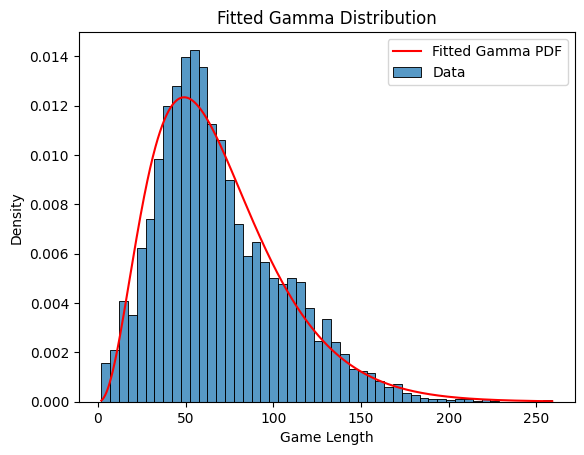
\includegraphics[width=0.8\linewidth]{gamma_fit.png}
    \caption{Gamma distribution fitted to the 'Turns' data}
    \label{fig:gamma_fit}
\end{figure}
\subsection{Distribution of 'Turns'}

To better understand the distribution of the 'Turns' variable, we attempted to fit it to several probability distribution families. The Gamma distribution was selected first due to its ability to model skewed data. However, as shown in Figure \ref{fig:gamma_fit}, the Gamma distribution is too broad for this dataset, suggesting it does not fully capture the underlying structure of 'Turns.'

To refine the fit, we combined the Gamma distribution with a Poisson distribution, which has a narrower shape. This combination results in a more accurate fit to the empirical data, as shown in Figure \ref{fig:gam_poi_fit}. The Gamma-Poisson mixture balances the excess spread of the Gamma distribution with the narrowness of the Poisson, providing a better representation of the 'Turns' distribution.



\begin{figure}[H]
    \centering
    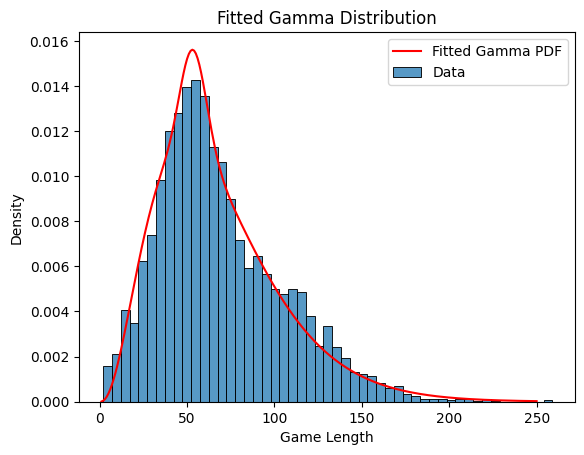
\includegraphics[width=0.8\linewidth]{gam_poi_fit.png}
    \caption{Gamma-Poisson distribution fitted to the 'Turns' data}
    \label{fig:gam_poi_fit}
\end{figure}



\newpage
\bibliographystyle{IEEEtran}
\bibliography{references}

\end{document}
